\begin{frame}{Solución}
La principal contribución es el desarrollo de una
heurística para acelerar la ejecución del
algoritmo K-means para grandes colecciones de datos
de alta dimensionalidad.

\begin{itemize}
\item Dado un conjunto de centroides, evitar el calculo
de distancia entre vectores, tomados por pares, para obtener una 
partición de la colección. Los autores proponen una asignación basada en el vecino más cercano de cada centroide.

\item Evitar el cálculo costoso detl verdadero centroide de 
cada cluster. Proponen una heurística para elegir el centroide
de una manera eficiente.
\end{itemize} 
\end{frame}

\begin{frame}{Heurísticas para el particionamiento rápido}

El principal cuello de botella del algoritmo K-means está
en la asignación de cada vector no centroide $d\in D - \cup_{k=1}^K$
a un cluster. Esto se logra eficientemente con la ayuda de la estructura
de datos \textbf{lista invertida}.

La lista invertida es particularmente adecuada para calcular
eficientemente el conjunto $TOP(x)$ para un vector dado $x$.
$TOP(x)$ nos da una lista de los vectores más similares
con respecto al vector actual $x$.

El algoritmo propuesto, \textbf{FPAC} (Fast PArtitional
Clustering), utiliza la heurística de vecino más cercano, es decir,
$TOP(x)$ como operación fundamental.

\end{frame}


\begin{frame}{Lista Invertida}
\begin{figure}
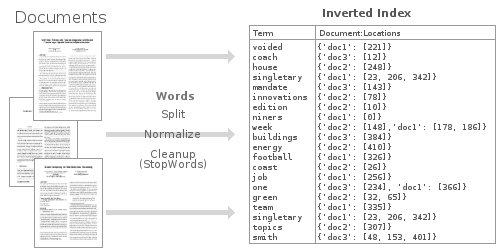
\includegraphics[scale=0.5]{img/invertedIndex}
\end{figure}
\end{frame}


\begin{frame}{Centroides como consultas}

Para asignar un vector no centroide $d$ a un cluster, se
usan los $K$ centroides como consultas. El objetivo es encontrar el 
conjunto de los vectores más cercanos (más similares), $TOP(x)$,
para cada centroide $x$. $TOP(C_k)$ del
centroide $C_k$ regresa 
una ranked list denotada por $L(C_k)$
% Si los centroides son diferentes entre ellos, es decir, no hay
% similitud en el contenido tópico, se espera que las ranked lists
% obtenidas de cada centroide, denotadas por $L(C_k)$,
% tengan una intersección pequeña.

\begin{itemize}
    \item Si un vector $d$  se obtiene del conjunto $TOP$ de sólo
una ranked list $L(C_k)$, se incluye en el conjunto de vectores
asignados al cluster correspondiente a $C_k$.
\item Si un vector $d$ se encuentra en múltiples ranked lists, se asigna
al cluster cuyo score normalizado de similitud es el máximo.
\end{itemize}


\begin{block}{¿Cuántos vectores deben recuperarse usando
cada centroide como consulta?}
Suponiendo una distribución uniforme de los 
vectores en los clusters, el número
promedio de vectores en cada cluster es $N/K$.
En el algoritmo FPAC se restringe el tamaño de
$TOP(x)$ a los $N/K$ vectores más similares.
\end{block}
\end{frame}


\begin{frame}{Centroides como consultas}
    \begin{figure}
        \centering
        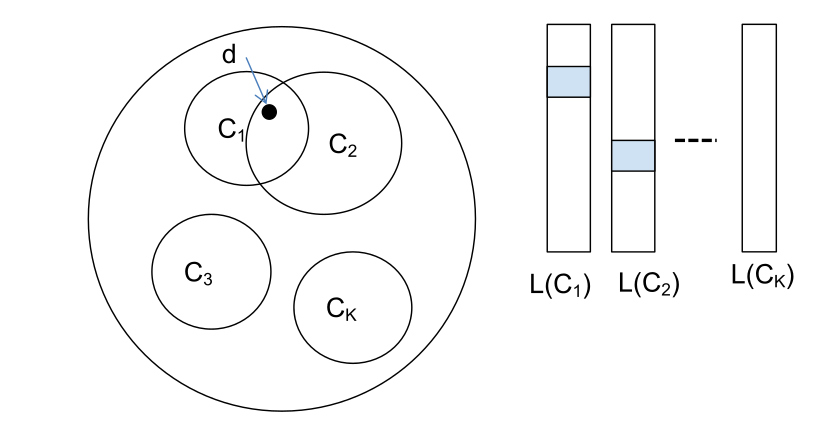
\includegraphics{img/cluster_example.jpg}
        \caption{K centroides $C_1, \dots, C_k$, son usados como consultas para obtener $K$ ranked lists de vectores, $L(C_1), L(C_2), \dots, L(C_k)$. Un
        vector $d$ es asignado a $C_1$ en vez
        de $C_2$ porque $d$ es más similar a $C_1$ que a $C_2$.}
    \end{figure}
\end{frame}


\begin{frame}{Selección de los centroides
iniciales}

Para asegurar que los centroides iniciales
son diferentes entre ellos, se selecciona el 
primer centroide $C_1$ aleatoriamente de toda
la colección. El siguiente centroide, $C_2$, 
se selecciona de tal forma que tenga una 
similitud muy baja con el centroide ya 
elegido. De manera más precisa, se formula 
una consulta utilizando 
los componentes del vector $C_1$.
$C_2$, se elige de manera aleatoria de un vector en la colección que no ocurra en la lista recuperada de $C_1$.
\end{frame}
\begin{frame}
\textbf{Agrupamiento de vectores no recuperados\\} 
Si un vector $d$ no es asignado a $\cup_{k=1}^K L(C_k)$ se asigna el vector
aleatoriamente a uno de los $k$ clusters.

\textbf{Recálculo de los centroides\\}
El algoritmo toma el vector con el máximo número de términos únicos dentro de un
cluster y lo actualiza como centroide.
\end{frame}